\begin{enumerate}[label=\thechapter.\arabic*,ref=\thechapter.\theenumi]
\item A damper with damping coefficient, $c$, is attached to a mass of $5$ \text{kg} and spring of stiffness  $5$ \text{kN/m} as shown in figure. The system undergoes under-damped oscillations.
If the ratio of the $3^{rd}$ amplitude to the $4^{th}$ amplitude of oscillations is ${1.5}$, the value of $c$ is ?
\begin{figure}[ht]
    \centering
    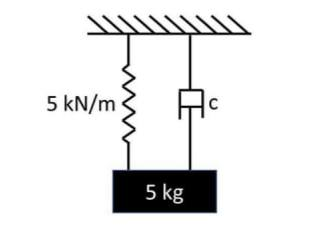
\includegraphics[width=\columnwidth]{2022/AE/62/figs/fig1.png}
\end{figure}

\hfill {(GATE AE-62 (2022))}
\solution
\newpage

\item A uniform rigid prismatic bar of total mass $ m$ is suspended from a ceiling by two
identical springs as shown in figure.
Let $ \omega_1$ and $ \omega_2$ be the natural frequencies of mode I and mode II respectively
($ \omega_1 < \omega_2$).
The value of $ \frac{\omega_2}{\omega_1}$ is \rule{1cm}{0.15mm} (rounded off to one decimal place).
\hfill(GATE AE 2022 QUESTION 63)\\
\begin{figure}[h!]
    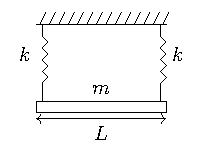
\includegraphics[width = \columnwidth]{2022/AE/63/figs/qn_fig.pdf}
    \caption{Figure given in question }
    \centering
    \label{fig: nm_63_fig_1}
\end{figure}
\solution
 \iffalse
\let\negmedspace\undefined
\let\negthickspace\undefined
\documentclass[journal,12pt,twocolumn]{IEEEtran}
\usepackage{cite}
\usepackage{amsmath,amssymb,amsfonts,amsthm}
\usepackage{algorithmic}
\usepackage{graphicx}
\usepackage{textcomp}
\usepackage{xcolor}
\usepackage{txfonts}
\usepackage{listings}
\usepackage{enumitem}
\usepackage{mathtools}
\usepackage{gensymb}
\usepackage{comment}
\usepackage[breaklinks=true]{hyperref}
\usepackage{tkz-euclide}
\usepackage{listings}
\usepackage{gvv}
\def\inputGnumericTable{}
\usepackage[latin1]{inputenc}
\usepackage{color}
\usepackage{array}
\usepackage{longtable}
\usepackage{calc}
\usepackage{multirow}
\usepackage{hhline}
\usepackage{ifthen}
\usepackage{lscape}

\newtheorem{theorem}{Theorem}[section]
\newtheorem{problem}{Problem}
\newtheorem{proposition}{Proposition}[section]
\newtheorem{lemma}{Lemma}[section]
\newtheorem{corollary}[theorem]{Corollary}
\newtheorem{example}{Example}[section]
\newtheorem{definition}[problem]{Definition}
\newcommand{\BEQA}{\begin{eqnarray}}
\newcommand{\EEQA}{\end{eqnarray}}
\newcommand{\define}{\stackrel{\triangle}{=}}
\theoremstyle{remark}
\newtheorem{rem}{Remark}
\begin{document}

\bibliographystyle{IEEEtran}
\vspace{3cm}

\title{GATE 2022  -AE 63}
\author{EE23BTECH11057 - Shakunaveti Sai Sri Ram Varun$^{}$% &lt;-this % stops a space
}
\maketitle
\newpage
\bigskip
\vspace{2cm}
\textbf{Question: }
A uniform rigid prismatic bar of total mass $ m$ is suspended from a ceiling by two
identical springs as shown in figure.
Let $ \omega_1$ and $ \omega_2$ be the natural frequencies of mode I and mode II respectively
($ \omega_1 < \omega_2$).
The value of $ \frac{\omega_2}{\omega_1}$ is \rule{1cm}{0.15mm} (rounded off to one decimal place).
\hfill(GATE AE 2022 QUESTION 63)\\
\begin{figure}[h!]
    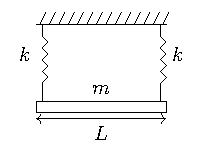
\includegraphics[width = \columnwidth]{2022/AE/63/figs/qn_fig.pdf}
    \caption{Figure given in question }
    \centering
    \label{fig: nm_63_fig_1}
\end{figure}

\textbf{Solution}:\\
\fi
\begin{table}[h!] 
\centering
\begin{tabular}{|c|c|c|}
    \hline
    \textbf{Parameter} & \textbf{Description} & \textbf{Value} \\
    \hline
    $X\brak{s}$ & position in laplace domain & $ X\brak{s}$ \\
    \hline
    $\Theta\brak{s}$ & angle rotated in laplace domain & $ \Theta\brak{s}$ \\
    \hline
    $x\brak{t}$ & position of mass w.r.t time & $x\brak{t}$ \\
    \hline
    $\theta\brak{t}$ & angle rotated by mass w.r.t time &$ \theta\brak{t}$\\
    \hline
    $\alpha\brak{t}$ & angular acceleration of mass w.r.t time & $\alpha\brak{t}$ \\
    \hline
    $k$ & spring constant & $ k$\\
    \hline
    $m$ & mass of the block & $ m$\\
    \hline
    $L$ & length of the mass & $ L$\\
    \hline
    $\omega_o$ & initial angular velocity of mass & $ \omega_o$ \\
    \hline
    $v\brak{0}$ & initial velocity of mass& $ v\brak{0}$ \\
    \hline
    
\end{tabular}






\caption{input values}
\label{tab: Table ae63}
\end{table}
\begin{enumerate}
    \item [\textbf{i:}] For vertical oscillations: from \figref{fig: nm_63_fig_2},
    \begin{align}
        m\frac{d^2x\brak{t}}{dt^2} + 2kx\brak{t} &=0
    \end{align}
    Assuming the bar is at mean position and has non-zero intitial velocity, we can write it's laplace transform as:
    \begin{align}
        s^2mX\brak{s}-mv\brak{0}+ 2kX\brak{s}&=0\\
        \implies X\brak{s} &= \frac{v\brak{0}}{s^2 + \frac{2k}{m}}
    \end{align}
    On taking inverse laplace transform we get,
    \begin{align}
        x\brak{t} &= v\brak{0}\sqrt{\frac{m}{2k}}\sin{\sqrt{\frac{2k}{m}}t}\\
        \therefore \omega_1 &= \sqrt{\frac{2k}{m}} \label{eq:gate63_1}
    \end{align}

\begin{figure}[h!]
    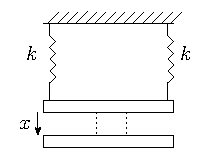
\includegraphics[width = \columnwidth]{2022/AE/63/figs/fig1.pdf}
    \caption{Figure for Vertical strain}
    \centering
    \label{fig: nm_63_fig_2}
\end{figure}

    \begin{figure}[h!]
    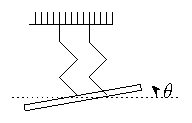
\includegraphics[width = \columnwidth]{2022/AE/63/figs/fig2.pdf}
    \caption{Figure for Torsional strain}
    \centering
    \label{fig: nm_63_fig_3}
\end{figure}
    \item [\textbf{ii:}] For torsional strain from \figref{fig: nm_63_fig_3},
    \begin{align}
        I\alpha\brak{t}&=-\frac{kL^2\theta\brak{t}}{2}
    \end{align}
Assuming it is at mean position and having non-zero angular velocity
we can write it's laplace transform as:
    \begin{align}
        s^2I\Theta\brak{s}-I\omega_o+ \frac{kL^2\Theta\brak{s}}{2}&=0
    \end{align}
    substituting values from \tabref{tab: Table ae63}:
    \begin{align}
        \Theta\brak{s}&=\frac{\omega_o}{s^2+\frac{6k}{m}}
    \end{align}
    On taking inverse laplace transform we get,
    \begin{align}
        \theta\brak{t} &= \omega_o\sqrt{\frac{m}{6k}}\sin{\sqrt{\frac{6k}{m}}t}\\
        \therefore \omega_2 &= \sqrt{\frac{6k}{m}} \label{eq:gate63_2}
    \end{align}
From \eqref{eq:gate63_1} and \eqref{eq:gate63_2} we see that
\begin{align}
    \frac{\omega_2}{\omega_1} &= \sqrt{3}
\end{align}








    
\end{enumerate}


\newpage

\end{enumerate}
